\chapter{Additional Results}\label{apx:results}
This appendix will present miscellaneous results not presented in the paper.
All executions presented in the results in this section are described in~\autoref{chp4:predictable_execution} unless else specified. 
Generally we have three different executions; CPU operations described in~\autoref{chp4:sec:microinstructions}, CPU load described in~\autoref{chp4:sec:cpu_load} and decryption described in~\autoref{chp4:sec:decryption}. 
We are working with two different microphone configurations, the portable setup and the lab grade setup, which is explained more in detail respectively in~\autoref{chp3:sec:knowles_configuration} and~\autoref{chp3:sec:bruel_kjaer_configuration}.

%==============
% Raspberry PI
%==============

\section{Raspberry PI}\label{apx:sec:raspberry}
All of our recordings of the Raspberry PI is more or less equal and inconclusive, empirically speaking. 
~\autoref{fig:appendix_RB-ekkofritt-bk-micro-0} is the inconclusive result gained from running the CPU operations. 
\begin{figure}[ht]
    \centering
    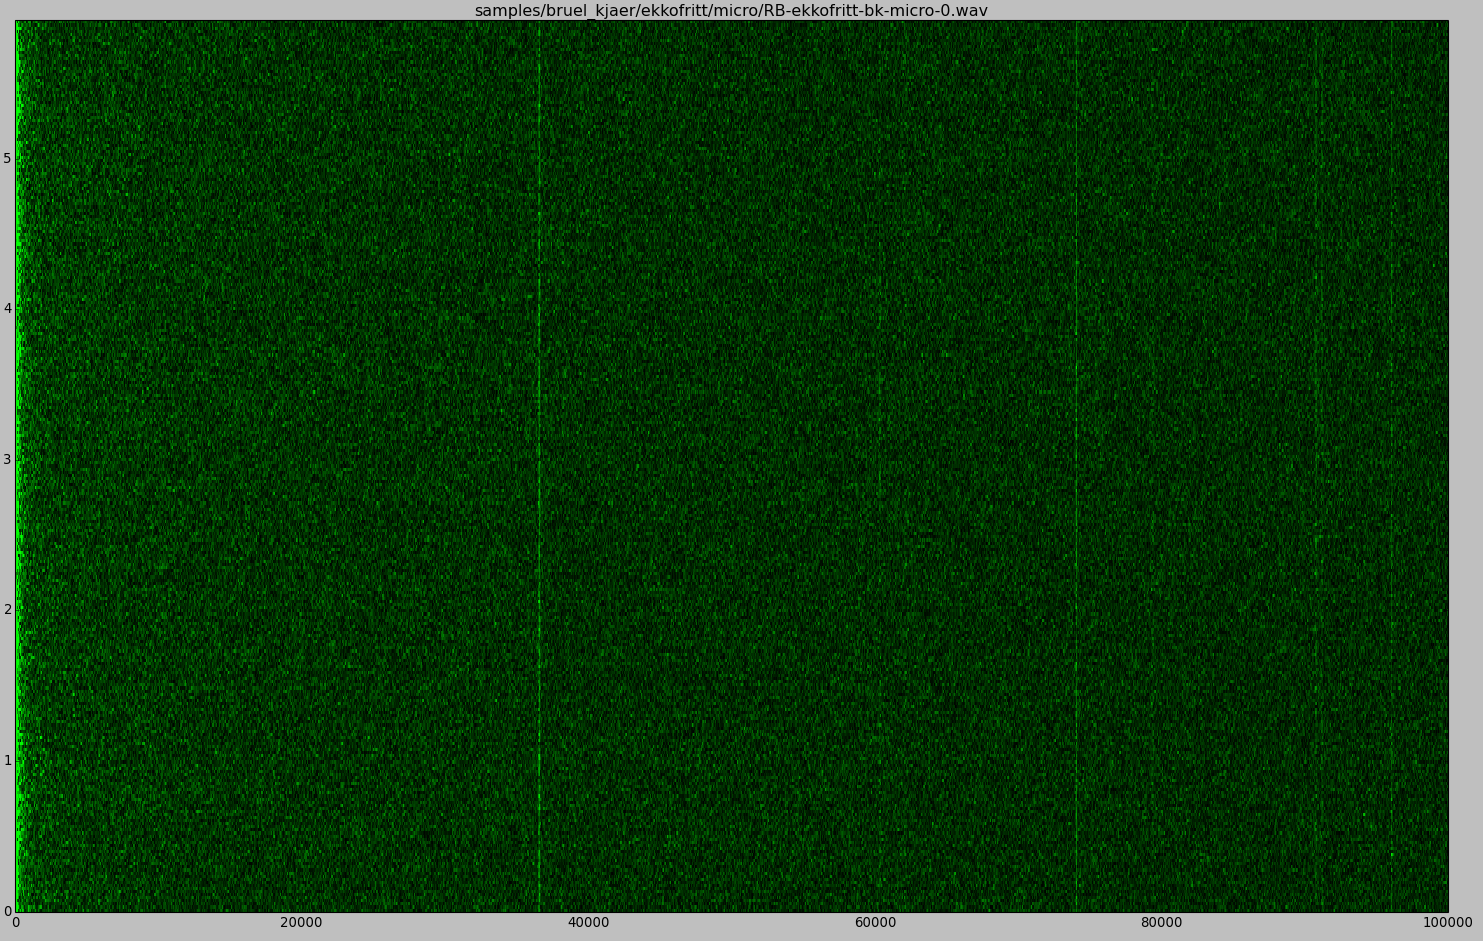
\includegraphics[width=1\linewidth]{RB-ekkofritt-bk-micro-0.png}
    \caption{Acoustic signature (6 sec, 0-100kHz) of the Raspberry PI running the CPU operations.
        Recorded in an anechoic chamber using the lab-grade setup.}
    \label{fig:appendix_RB-ekkofritt-bk-micro-0}
\end{figure}


%==========================
% T60p Normal room CPULOAD
%==========================
\section{Normal office environment}

~\autoref{fig:appendix_T60p-bk-cpuload-eps-1-1a} and~\autoref{fig:appendix_T60p-bk-cpuload-ips-0-1b} is the results from the running CPU load on the Lenovo T60p in an office environment. 
\begin{figure}[ht]
	\begin{subfigure}{1\textwidth}
	    \centering
	    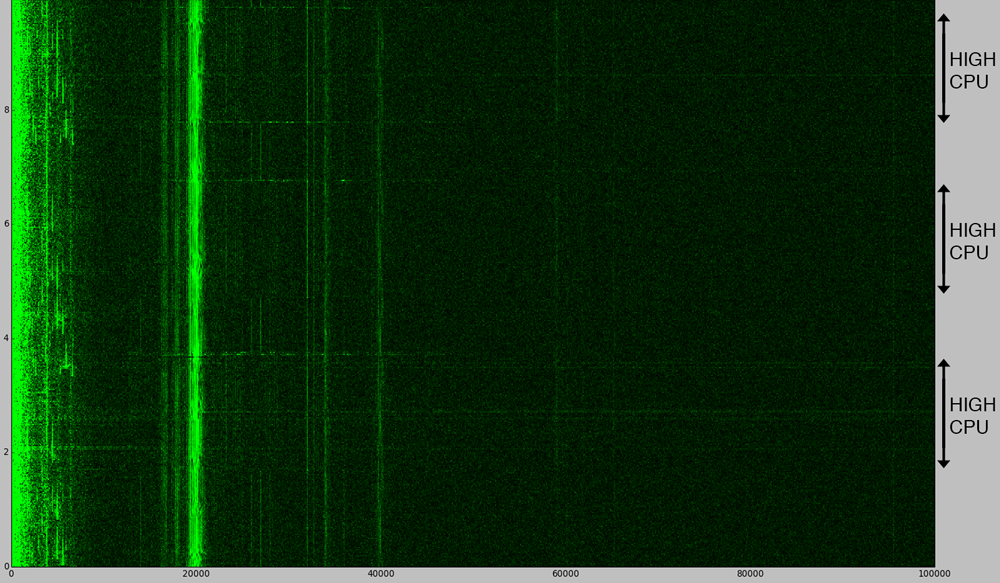
\includegraphics[width=1\linewidth]{T60p-bk-cpuload-eps-1_description.png}
	    \caption{With AC power adopter}
	    \label{fig:appendix_T60p-bk-cpuload-eps-1-1a}
    \end{subfigure}
    \begin{subfigure}{1\textwidth}
	    \centering
	    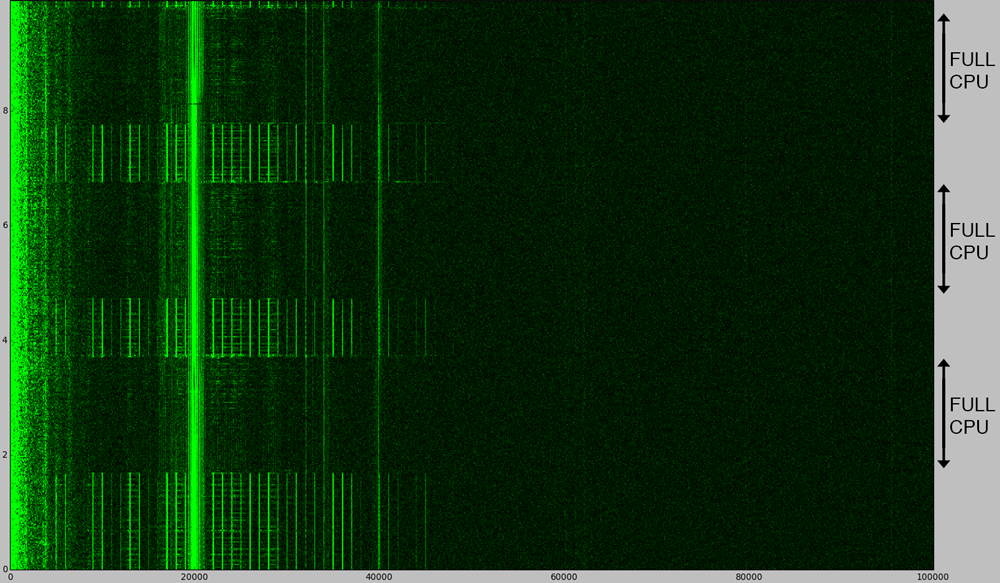
\includegraphics[width=1\linewidth]{T60p-bk-cpuload-ips-0_description.png}
	    \caption{Running on battery power}
	    \label{fig:appendix_T60p-bk-cpuload-ips-0-1b}
    \end{subfigure}
    \caption{Acoustic signature (10 sec, 0-100kHz) of the Lenovo T60p when running a high CPU load described in~\autoref{chp4:sec:cpu_load}. Recorded in an anechoic chamber using the lab-grade setup. }
	\label{fig:appendix_T60p-bk-cpuload}
\end{figure}

%=============================
% D430 Anechoic chamber  IDLE
%=============================
%The~\autoref{fig:D430-ekkofritt-bk-idle-eps-1} is the result from the running idle on the Dell 430 in the anechoic chamber. 
%\begin{figure}[ht]
%    \centering
%    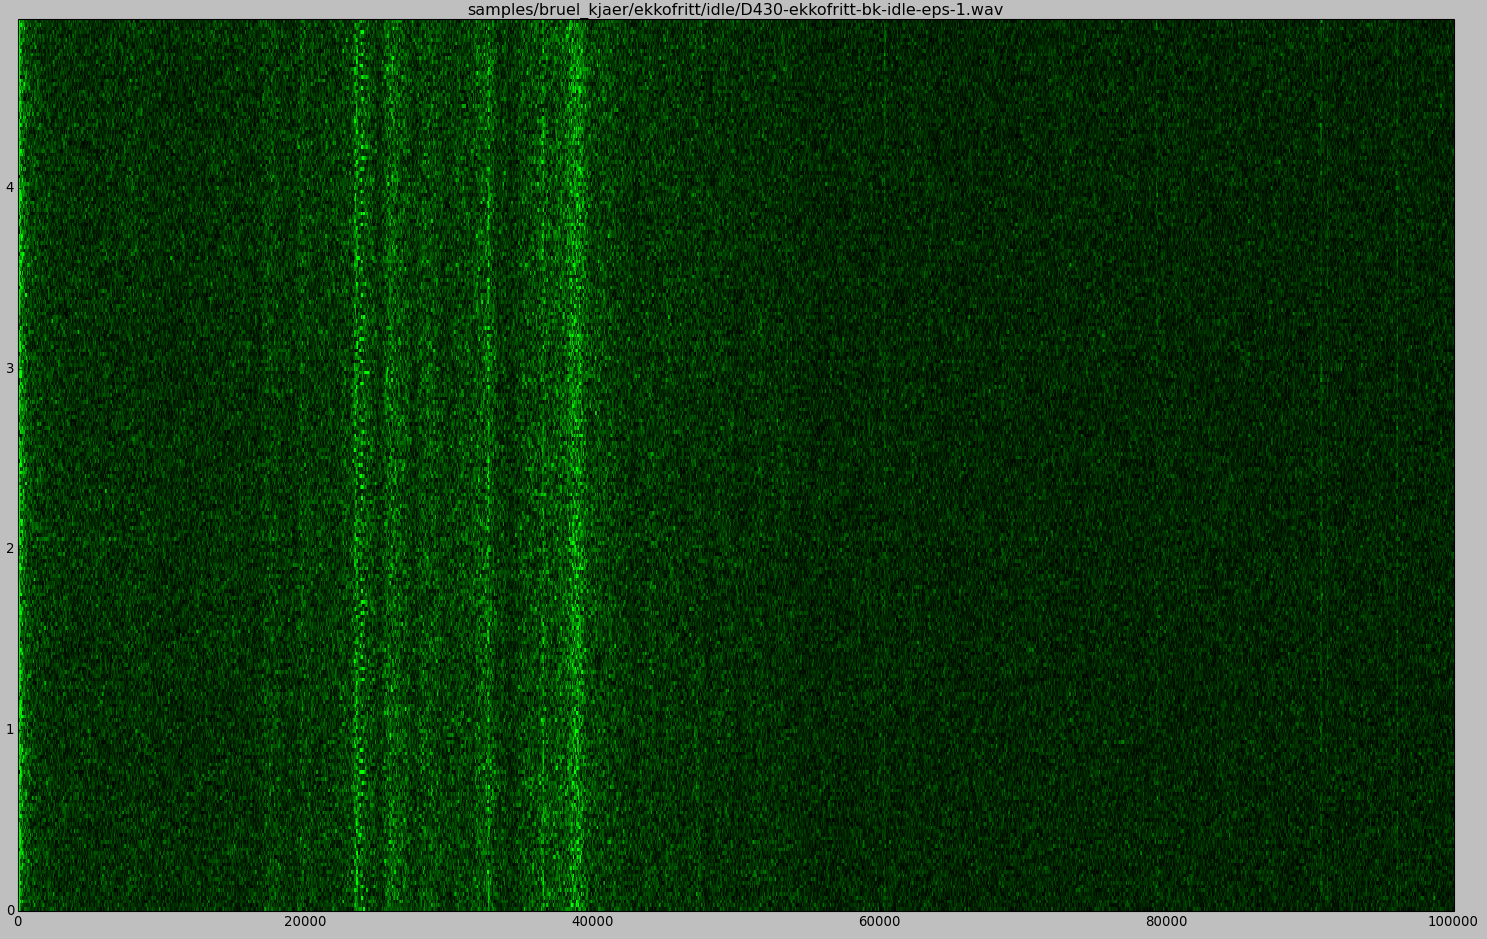
\includegraphics[width=0.7\linewidth]{D430-ekkofritt-bk-idle-eps-1.png}
%    \caption{Acoustic recording (Vertical axis: 5 sec. Horizontal axis: 0-100kHz) of the Dell D430 when idle. The recording was made in an anechoic chamber using the Brüel\&Kjær 4939 configuration specified in~\autoref{chp3:sec:bruel_kjaer_configuration}. }
%    \label{fig:D430-ekkofritt-bk-idle-eps-1}
%\end{figure}

